\documentclass[10pt]{beamer}
\usepackage[T1]{fontenc}
\usepackage[utf8]{inputenc}
\usepackage[french]{babel}
\usepackage{color}
\usepackage[normalem]{ ulem }
\usepackage{soul}
\usetheme{Darmstadt}

\title{Les projets ATM2 et SAVOIE}
\subtitle{Formation à destination du superviseur}
\author{Clovis HAMEL, Lo\"{i}c PERRIN, Michael AMAND}
\date{\today}

\AtBeginSubsection[]
{
  \begin{frame}<beamer>{Plan}
    \tableofcontents[currentsection,currentsubsection]
  \end{frame}
}

% Let's get started
\begin{document}

\begin{frame}
  \titlepage
\end{frame}

\begin{frame}{}
  \tableofcontents
  % You might wish to add the option [pausesections]
\end{frame}

%%%%%%%%%%%%%%%%%%%%%%%%%%%%%%%%%%%%%%%%%%%
\section{Introduction}
%%%%%%%%%%%%%%%%%%%%%%%%%%%%%%%%%%%%%%%%%%%

\begin{frame}{Une prise de conscience nécessaire 1/2}
\begin{block}{Évolution des architectures applicatives}
\begin{itemize}
\item Applications client-serveur légers \pause
\item Recours aux technologies Web 2.0 (PHP, Javascript, Bootstrap, etc) \pause
\item Recours aux API (B2B Network Manager par exemple) \pause
\item Utilisation de technologies de conteneurisation telles que Docker \pause
\end{itemize}
\end{block}
\begin{block}{Évolution des méthodes de développement}
\begin{itemize}
\item Mise en retrait de la DTI \pause
\item Cycle de développement et de déploiement plus courts (cf ASAP, itérativité, etc) \pause
\item Diminution des RH mais contraintes maintenues \pause
\end{itemize}
\end{block}
\end{frame}

\begin{frame}{Une prise de conscience nécessaire 2/2}
\begin{block}{Evolution des méthodes de gestion de projet}
\begin{itemize}
\item Eviter l'effet tunnel en livrant plus souvent \pause
\item Déployer en continu \pause
\item Automatiser les tests (cf gitlab) \pause
\item Conserver une disponibilité maximum (sur panne et sur déploiement) par un retour arrière natif \pause
\end{itemize}
\end{block}
\end{frame}

\begin{frame}{Une dette technologique à combler}
\begin{block}{Un contrôle aérien qui a soif de modernité}
\begin{itemize}
    \item Décloisonnement des acteurs du TA (PC, FMP, CDS, Cie, NM, etc) \pause
    \item Numérisation et automatisation de l'information (\sout{téléphone})
    \item Une vitrine pour valoriser les compétences internes de la DSNA 
\end{itemize}
\end{block} 
 \begin{exampleblock}{Exemples d'applicatifs}
 WikiFF, 4Me, SALTO (sur SAVOIE), iStream, CCS (sur leur propre machines)
\end{exampleblock}
\begin{block}{Un existant peu optimal}
\begin{itemize}
\item Un bi-serveur par application (SIAM, EPEIRES, WikiFF)
\item Une box Internet par applicatif (iSTREAM, SALTO, etc)
\item Aucune mutualisation des services (3 applications sur SIAM-TECH, 3 serveurs MySQL)
\item Chaque section doit se former sur des méthodes de travail similaires 
\end{itemize}
\end{block}
\end{frame}

%%%%%%%%%%%%%%%%%%%%%%%%%%%%%
% Les solutions
%%%%%%%%%%%%%%%%%%%%%%%%%%%%%
\begin{frame}{Une solution en deux temps}
\begin{block}{Deux salles, deux ambiances, un même plaisir}
\begin{itemize}
    \item Une solution nationale : Le réseau ATM2 
    \item Une solution locale : L'infrastructure SAVOIE
\end{itemize}
\end{block} 

\begin{alertblock}{Nécessité de différencier les deux}
\begin{itemize}
    \item Pas les mêmes matériels
    \item Pas les mêmes intervenants nationaux et locaux impliqués
\end{itemize}
\end{alertblock} 

\begin{alertblock}{Mais les deux ne sont pas bijectifs ! \#ClassePrepa}
\begin{itemize}
    \item SAVOIE nécessite forcément ATM2 a priori ... \footnote{vSphere ne sert pas à virtualiser des clients. On peut le faire si on veut mais ce n'est pas fait pour. Au premier ordre, si on utilise SAVOIE pour implémenter un système, on utilisera ATM2. Si on ne veut pas utiliser ATM2, on utilise une infra indépendante.}
    \item Mais on peut connecter des systèmes sur ATM2 sans utiliser l'infrastructure SAVOIE. 
\end{itemize}
\end{alertblock} 
\end{frame}

%%%%%%%%%%%%%%%%%%%%%%%%%%%%%%%%%%%%%%%%%%%
\section{ATM2}
%%%%%%%%%%%%%%%%%%%%%%%%%%%%%%%%%%%%%%%%%%%
cf. Cours de Mickael Papail

%%%%%%%%%%%%%%%%%%%%%%%%%%%%%%%%%%%%%%%%%%%
\section{SAVOIE}
%%%%%%%%%%%%%%%%%%%%%%%%%%%%%%%%%%%%%%%%%%%
%%%%%%%%%%%%%%%%%%%%%%%%%%%%%
% Qu'est ce que SAVOIE ?
%%%%%%%%%%%%%%%%%%%%%%%%%%%%%

\begin{frame}{SAVOIE bien ou quoi ?}
\begin{block}{SAVOIE}
\begin{itemize}
\item Solution d’Architecture Virtuelle pour l’Opérationnel, Innovante et Évolutive
\item Solution all-in-one d'hébergement à la sauce OVH, AWS
\item Solution locale désignée par l'équipe projet CRNA/N ATM2
\end{itemize}
\end{block}
\begin{block}{Forces de l'infrastructure}
\begin{itemize}
\item Cluster de machines \pause
\item Virtualisation des applicatifs \pause
\item Stockage partagé sur SAN \pause 
\end{itemize}
\end{block}
\end{frame}

\begin{center}
\begin{frame}{Schéma d'infrastructure SAVOIE}
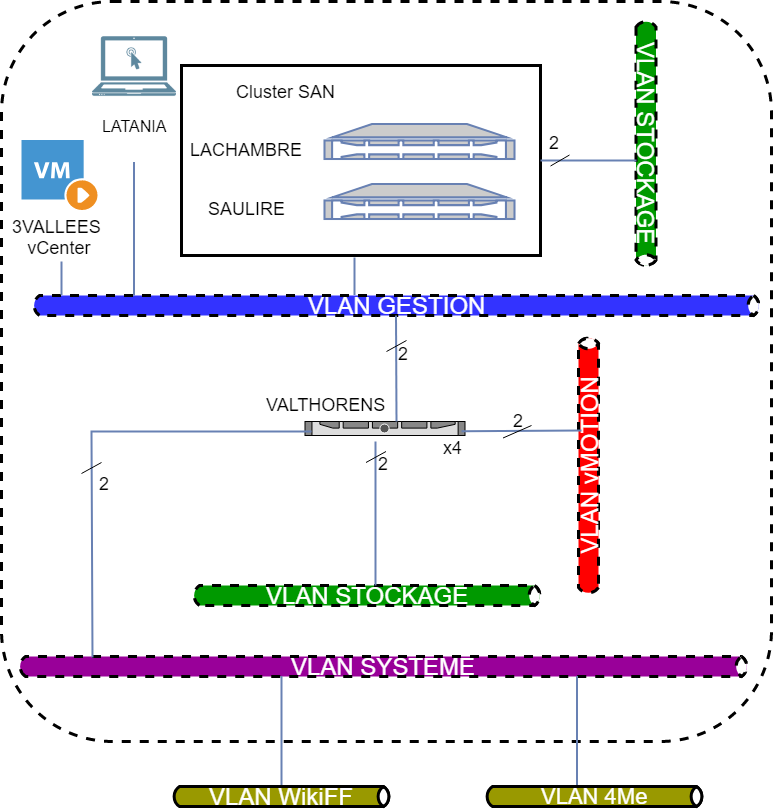
\includegraphics[width=200px]{Schemas/SAVOIE.png}
\end{frame}
\end{center}

\subsection{La virtualisation}



\subsection{Les fonctionnalités VMware}

\begin{center}
\begin{frame}{vMotion}
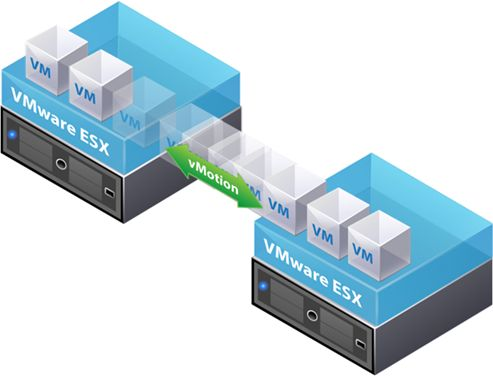
\includegraphics[width=260px]{Schemas/vMotion.jpg}
\end{frame}
\end{center}

\begin{center}
\begin{frame}{Storage vMotion}
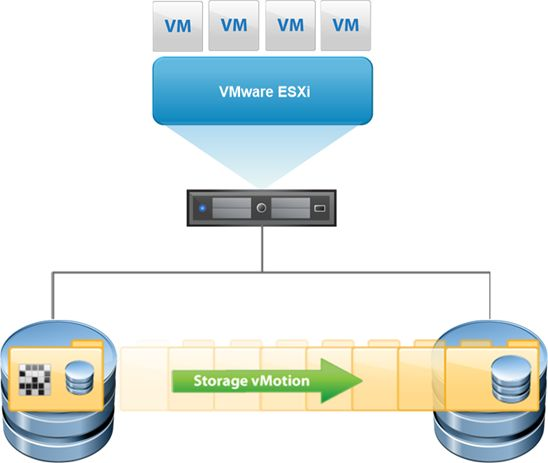
\includegraphics[width=250px]{Schemas/Storage_vMotion.jpg}
\end{frame}
\end{center}

\begin{center}
\begin{frame}{Thin Provisionning vs Thick Provisionning}
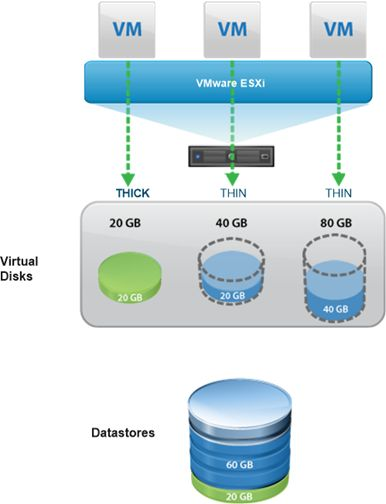
\includegraphics[width=150px]{Schemas/Thin_Provisionning.jpg}
\end{frame}
\end{center}

\begin{center}
\begin{frame}{High Availability (HA)}
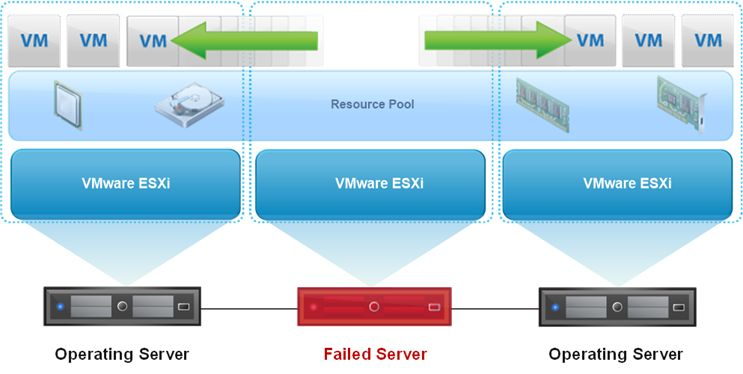
\includegraphics[width=310px]{Schemas/High_Aviability.jpg}
\end{frame}
\end{center}

\begin{center}
\begin{frame}{Fault Tolerance (FT)}
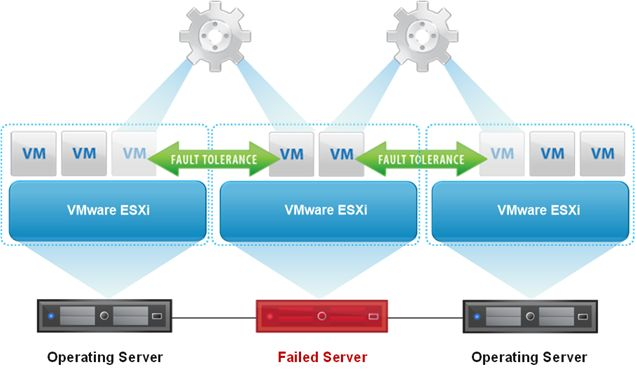
\includegraphics[width=310px]{Schemas/Fault_Tolerance.jpg}
\end{frame}
\end{center}

\begin{frame}{Isolation des flux}
\begin{block}{Quatre VLAN tagués sont utilisés}
\begin{itemize}
\item GESTION pour administrer les ESX et les SAN via un poste d'administration (LATANIA)
\item vMOTION pour la migration des VM d'un ESX à un autre
\item STOCKAGE pour les lectures et écritures sur le SAN
\item SYSTEME sur lequel les VM applicatives serveurs communiquent avec les clients physiques
\end{itemize}
\end{block}
\begin{block}{Pourquoi isoler les flux ?}
\begin{itemize}
    \item Préconisation de l'ANSSI
    \item Allocation de ressources indépendantes et dédiées.
\end{itemize}
\end{block}
\begin{exampleblock}{Exemple}
Un VLAN GESTION a besoin de beaucoup moins de ressources qu'un VLAN STOCKAGE
\end{exampleblock}
\end{frame}

\begin{frame}{Vu de l'ESX}
\includegraphics[width=300px]{Schemas/VLAN.png}
\end{frame}

%%%%% A faire
%\begin{frame}{Vu du SAN}
%\includegraphics[width=300px]{VLAN.png}
%\end{frame}



\begin{center}
\begin{frame}{Maquettage de la baie SAVOIE}
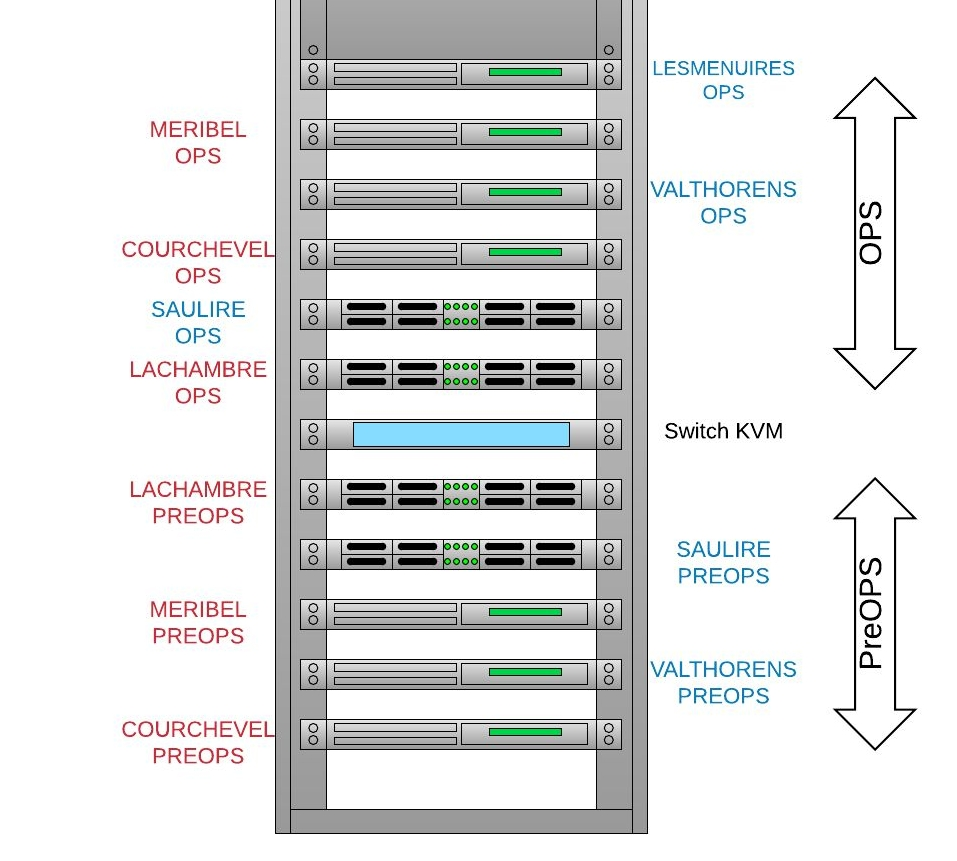
\includegraphics[width=250px]{Schemas/Maquettage_Savoie.jpg}
\end{frame}
\end{center}

%%%%%%%%%%%%%%%%%%%%%%%%%%%%%%%%%%%%%%%%%%%
\section{Maintenance Opérationnelle}
%%%%%%%%%%%%%%%%%%%%%%%%%%%%%%%%%%%%%%%%%%%
\begin{frame}{Qui assure la MO de ATM2 et SAVOIE ?}
\begin{block}{Une MO répartie sur deux superviseurs}
\begin{itemize}
\item Les superviseurs RVU (resp CAW) utilisent leur casquette ODR (resp WAN) pour superviser le réseau ATM2
\item Les superviseurs RVU (resp CAW) utilisent leur casquette ODA (resp CAU) pour superviser SAVOIE
\end{itemize}
\end{block}
\begin{alertblock}{Attention}
\begin{itemize}
    \item Le réseau ATM2 n'est pas supervisé par la MO en 2018
    \item Il est supervisé par la MS ODR et WAN conjointement 
\end{itemize}
\end{alertblock}
\end{frame}

\begin{frame}{Que doit faire le superviseur ?}
\begin{block}{Processus en trois temps}
\begin{itemize}
\item Identifier
\item Communiquer
\item Agir
\end{itemize}
\end{block}
\begin{block}{Outils à la disposition des superviseurs}
\begin{itemize}
\item La station d'administration LATANIA
\item La supervision (??)
\item SIAM 
\end{itemize}
\end{block}
\end{frame}

\begin{frame}{Identifier et Communiquer}
\begin{block}{Identifier l'incident}
\begin{itemize}
\item Identifier une panne de composants réseaux (switch) ou applicatifs (ESX, disque, etc)
\item Identifier un vMotion réalisé par vSphere (??)
\end{itemize}
\end{block}
\begin{block}{Communiquer}
\begin{itemize}
\item Aux utilisateurs et à la MS l'impact et le temps de rétablissement
\end{itemize}
\end{block}
\end{frame}

\begin{frame}{Agir}
\begin{block}{Agir sur une VM}
\begin{itemize}
\item Arrêter/Démarrer une VM dégradée ou en panne
\end{itemize}
\end{block}
\begin{block}{Agir sur les ESX}
\begin{itemize}
\item \textcolor{red}{Aucun changement d'ESX n'est fait par la MO}
\end{itemize}
\end{block}
\begin{block}{Agir sur les SAN}
\begin{itemize}
\item \textcolor{red}{Aucun changement de disque SAN n'est fait par la MO}
\item \textcolor{red}{Aucun changement de SAN n'est fait par la MO}
\end{itemize}
\end{block}
\end{frame}

\end{document}